\documentclass{article}
\usepackage[utf8]{inputenc}
\usepackage{tikz}
\usepackage{pgfplots}
\pgfplotsset{compat=1.18}
\usetikzlibrary{shapes,arrows,positioning,decorations.pathreplacing}

\title{TikZ Diagrams in LaTeX}
\author{Your Name}
\date{\today}

\begin{document}

\maketitle

\section{Basic TikZ Examples}
Here are some basic TikZ diagrams:

\subsection{Simple Shapes}
\begin{tikzpicture}
% Draw a circle
\draw (0,0) circle (1cm);

% Draw a rectangle
\draw (3,0) rectangle (5,2);

% Draw a line
\draw (6,0) -- (8,2);

% Draw an arrow
\draw[->] (9,0) -- (11,2);
\end{tikzpicture}

\subsection{Coordinate System}
\begin{tikzpicture}
% Draw axes
\draw[->] (0,0) -- (4,0) node[right] {$x$};
\draw[->] (0,0) -- (0,4) node[above] {$y$};

% Draw points
\fill (1,1) circle (2pt) node[below right] {$(1,1)$};
\fill (3,2) circle (2pt) node[above left] {$(3,2)$};

% Draw line between points
\draw (1,1) -- (3,2);
\end{tikzpicture}

\section{Flowcharts}
Here's a simple flowchart:

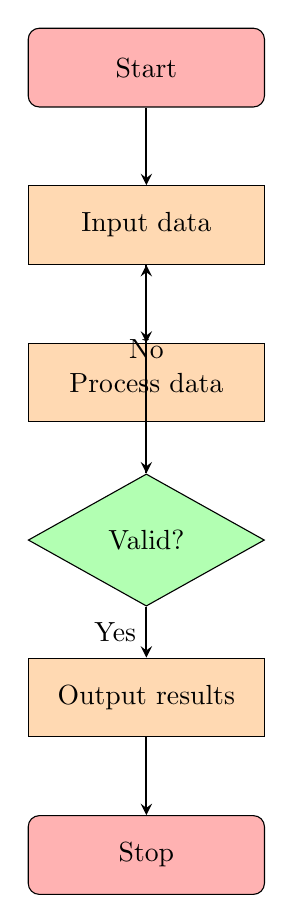
\begin{tikzpicture}[node distance=2cm]
% Define styles
\tikzstyle{startstop} = [rectangle, rounded corners, minimum width=3cm, minimum height=1cm, text centered, draw=black, fill=red!30]
\tikzstyle{process} = [rectangle, minimum width=3cm, minimum height=1cm, text centered, draw=black, fill=orange!30]
\tikzstyle{decision} = [diamond, minimum width=3cm, minimum height=1cm, text centered, draw=black, fill=green!30]
\tikzstyle{arrow} = [thick,->,>=stealth]

% Draw nodes
\node (start) [startstop] {Start};
\node (input) [process, below of=start] {Input data};
\node (process) [process, below of=input] {Process data};
\node (decision) [decision, below of=process] {Valid?};
\node (output) [process, below of=decision] {Output results};
\node (stop) [startstop, below of=output] {Stop};

% Draw arrows
\draw [arrow] (start) -- (input);
\draw [arrow] (input) -- (process);
\draw [arrow] (process) -- (decision);
\draw [arrow] (decision) -- node[anchor=east] {Yes} (output);
\draw [arrow] (decision) -- node[anchor=south] {No} (input);
\draw [arrow] (output) -- (stop);
\end{tikzpicture}

\section{Mathematical Plots}
Here's a mathematical plot:

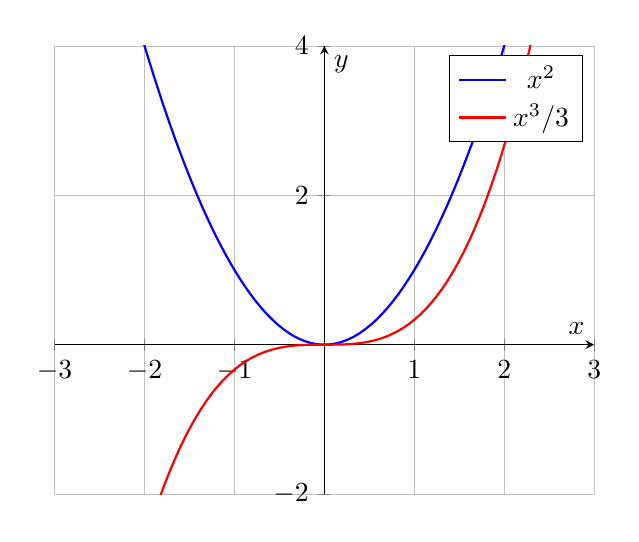
\begin{tikzpicture}
\begin{axis}[
    axis lines = center,
    xlabel = $x$,
    ylabel = $y$,
    xmin = -3, xmax = 3,
    ymin = -2, ymax = 4,
    grid = both,
    grid style = {line width=.1pt, draw=gray!10},
    major grid style = {line width=.2pt, draw=gray!50},
]
\addplot[domain=-3:3, samples=100, color=blue, thick] {x^2};
\addplot[domain=-3:3, samples=100, color=red, thick] {x^3/3};
\legend{$x^2$, $x^3/3$}
\end{axis}
\end{tikzpicture}

\section{Network Diagrams}
Here's a simple network diagram:

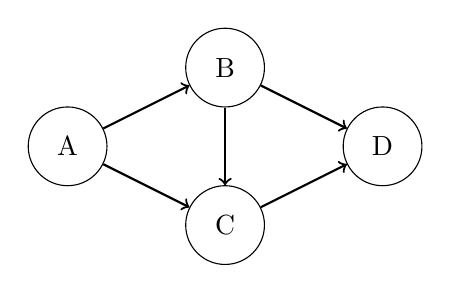
\begin{tikzpicture}[node distance=2cm]
% Define node styles
\tikzstyle{node} = [circle, draw, minimum size=1cm]
\tikzstyle{edge} = [thick, ->]

% Draw nodes
\node[node] (A) at (0,0) {A};
\node[node] (B) at (2,1) {B};
\node[node] (C) at (2,-1) {C};
\node[node] (D) at (4,0) {D};

% Draw edges
\draw[edge] (A) -- (B);
\draw[edge] (A) -- (C);
\draw[edge] (B) -- (D);
\draw[edge] (C) -- (D);
\draw[edge] (B) -- (C);
\end{tikzpicture}

\section{Advanced TikZ Features}
Here are some advanced TikZ features:

\subsection{Decorations}
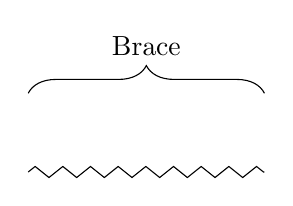
\begin{tikzpicture}
\draw[decorate, decoration={brace, amplitude=10pt}] (0,0) -- (3,0) node[midway, above=10pt] {Brace};
\draw[decorate, decoration={zigzag, amplitude=2pt}] (0,-1) -- (3,-1);
\end{tikzpicture}

\subsection{Shadows and Effects}

\begin{tikzpicture}
% Simulated drop shadow using a filled, slightly offset rectangle
\fill[black, opacity=0.3] (0.1,-0.1) rectangle (2.1,0.9);
\draw[fill=blue!20, draw=blue, thick] (0,0) rectangle (2,1);
\end{tikzpicture}

\section{Best Practices for TikZ}
\begin{itemize}
    \item Use relative coordinates when possible
    \item Define styles for consistent formatting
    \item Use meaningful node names
    \item Keep diagrams simple and clear
    \item Use appropriate line weights and colors
    \item Test diagrams at different scales
\end{itemize}

\end{document}
